%------------------------------------------------------------------------------
% Ashish Reddy Ette -- Full Stack Software Engineer Resume (v2, modern layout)
% Design goals: 7-second scan, ATS-safe single column, strong visual hierarchy
%   - Full-bleed header band -> impact metrics strip -> short quantified bullets
%   - Generous margins / line spacing, one accent colour, real text (no images)
% Build: xelatex resume.tex  (run twice: header band uses overlay positioning)
%------------------------------------------------------------------------------

\documentclass[a4paper,10pt]{article}

\usepackage{fontspec}
\setmainfont{Inter}[
  UprightFont    = *,
  BoldFont       = * SemiBold,
  ItalicFont     = * Italic,
  BoldItalicFont = * SemiBold Italic,
  RawFeature     = {-calt;-ccmp}  % contextual alternates break PDF text mapping (+ ( ) vanish for ATS)
]
\newfontfamily\headerfontbase{Inter Display}[
  UprightFont = *,
  BoldFont    = * Bold,
  RawFeature  = {-calt;-ccmp}
]
\newcommand{\headerfont}{\headerfontbase\bfseries}
\newfontfamily{\faSolid}[Path=/usr/share/fonts/fontawesome-7-free-fonts/]{Font Awesome 7 Free-Solid-900.otf}
\newfontfamily{\faBrands}[Path=/usr/share/fonts/fontawesome-7-brands-fonts/]{Font Awesome 7 Brands-Regular-400.otf}
\newcommand{\iconPhone}{{\faSolid\symbol{"F095}}}
\newcommand{\iconEmail}{{\faSolid\symbol{"F0E0}}}
\newcommand{\iconLocation}{{\faSolid\symbol{"F3C5}}}
\newcommand{\iconLinkedIn}{{\faBrands\symbol{"F08C}}}
\newcommand{\iconGitHub}{{\faBrands\symbol{"F09B}}}
\newcommand{\iconExternal}{{\faSolid\symbol{"F08E}}}
\newcommand{\iconStar}{{\faSolid\symbol{"F005}}}
\newcommand{\iconCert}{{\faSolid\symbol{"F559}}}

% --- Colour palette: deep navy + one blue accent ----------------------------
\usepackage[dvipsnames,svgnames,x11names]{xcolor}
\definecolor{Navy}{HTML}{0B1F3A}        % header band
\definecolor{Accent}{HTML}{2563EB}      % section titles, bullets, metrics
\definecolor{AccentSoft}{HTML}{93C5FD}  % job title on the dark band
\definecolor{PrimaryText}{HTML}{0F172A} % headings
\definecolor{BodyText}{HTML}{1E293B}    % body copy (high contrast)
\definecolor{MutedText}{HTML}{64748B}   % dates / locations
\definecolor{Rule}{HTML}{E2E8F0}        % hairlines
\definecolor{Tint}{HTML}{F1F5F9}        % metrics strip background

% --- Page geometry: real margins, breathing room ----------------------------
\usepackage[top=0.4in, bottom=0.45in, left=0.7in, right=0.7in]{geometry}
\pagestyle{empty}
\raggedbottom
\raggedright
\setlength{\parindent}{0pt}
\linespread{1.1}

\usepackage[hidelinks]{hyperref}
\hypersetup{
  colorlinks=true, linkcolor=Accent, urlcolor=Accent,
  pdftitle={Ashish Reddy Ette - Resume},
  pdfauthor={Ashish Reddy Ette}
}
\urlstyle{same}

\usepackage{enumitem}
\usepackage{array}
\usepackage{tikz}
\usetikzlibrary{calc}

% --- Bullets ----------------------------------------------------------------
\newcommand{\resumebullet}{%
  \tikz[baseline=-0.45ex]\fill[Accent] (0,0) circle (1.3pt);%
}
\newlist{resumeList}{itemize}{1}
\setlist[resumeList]{
  label=\resumebullet, leftmargin=1.2em,
  itemsep=3.4pt, parsep=0pt, topsep=3pt, partopsep=0pt
}

% --- Section heading: letter-spaced caps + hairline --------------------------
\newcommand{\resumeSection}[1]{%
  \vspace{12pt}%
  \noindent{\addfontfeature{LetterSpace=9}\fontsize{9.6}{12}\selectfont\headerfont\color{Accent}\MakeUppercase{#1}}%
  \hspace{8pt}{\color{Rule}\leaders\hrule height 0.8pt\hfill\kern0pt}\par
  \vspace{5pt}%
}

% --- Role / school heading ----------------------------------------------------
\newcommand{\roleHeading}[4]{%
  \noindent\begin{tabular*}{\linewidth}{@{}l@{\extracolsep{\fill}}r@{}}
    {\fontsize{11}{14}\selectfont\bfseries\color{PrimaryText}#1} & {\small\color{MutedText}#2}\\
    {\small\bfseries\color{Accent}#3} & {\small\color{MutedText}#4}
  \end{tabular*}\par\vspace{1pt}%
}

% --- Metric tile ------------------------------------------------------------
\newcommand{\metric}[2]{%
  \begin{tabular}[c]{@{}c@{}}
    {\fontsize{17}{19}\selectfont\headerfont\color{Accent}#1}\\[1pt]
    {\fontsize{8}{10}\selectfont\color{MutedText}#2}
  \end{tabular}%
}

\begin{document}
\color{BodyText}

%==============================================================================
% HEADER BAND (full bleed)
%==============================================================================
\begin{tikzpicture}[remember picture, overlay]
  \fill[Navy] (current page.north west) rectangle ([yshift=-3.0cm]current page.north east);
  \fill[Accent] ([yshift=-3.0cm]current page.north west) rectangle ([yshift=-3.1cm]current page.north east);
  \node[anchor=north west, inner sep=0pt, text width=\textwidth]
    at ([xshift=0.7in, yshift=-0.6cm]current page.north west) {%
    \raggedright
    {\fontsize{29}{33}\selectfont\headerfont\color{white}Ashish Reddy Ette}\\[4pt]
    {\fontsize{12}{15}\selectfont\bfseries\color{AccentSoft}Full Stack Software Engineer}%
    {\fontsize{12}{15}\selectfont\color{white!55!Navy}\quad|\quad}%
    {\fontsize{10.5}{15}\selectfont\color{white!85!Navy}Java \textperiodcentered\ Spring Boot \textperiodcentered\ Angular}\hfill{\fontsize{9.5}{15}\selectfont\color{white!85!Navy}\iconLocation\ \ Hyderabad, India}\\[9pt]
    {\fontsize{9}{12}\selectfont\color{white}%
      \href{tel:+918106026438}{\color{white}\iconPhone\ \ +91 8106026438}\hfill%
      \href{mailto:etteashishreddy1504@gmail.com}{\color{white}\iconEmail\ \ etteashishreddy1504@gmail.com}\hfill%
      \href{https://www.linkedin.com/in/ashish-reddy-ette-5286a1196/}{\color{white}\iconLinkedIn\ \ ashish-reddy-ette}\hfill%
      \href{https://github.com/ashishreddy-15}{\color{white}\iconGitHub\ \ ashishreddy-15}%
    }%
  };
\end{tikzpicture}
\vspace*{1.95cm}

%==============================================================================
% IMPACT METRICS STRIP
%==============================================================================
\noindent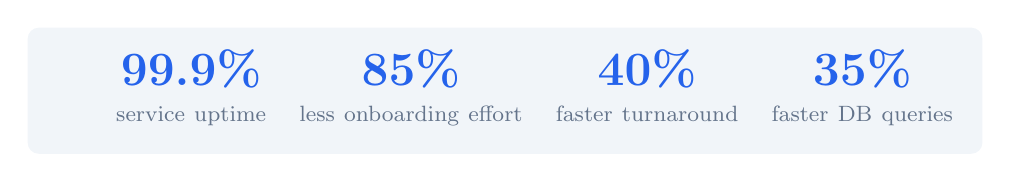
\begin{tikzpicture}
  \node[fill=Tint, rounded corners=4pt, inner xsep=16pt, inner ysep=8pt, text width=\dimexpr\linewidth-32pt\relax, align=center] {%
    \begin{tabular*}{\dimexpr\linewidth-32pt\relax}{@{\extracolsep{\fill}}c c c c@{}}
      \metric{99.9\%}{service uptime} &
      \metric{85\%}{less onboarding effort} &
      \metric{40\%}{faster turnaround} &
      \metric{35\%}{faster DB queries}
    \end{tabular*}
  };
\end{tikzpicture}

%==============================================================================
% SUMMARY
%==============================================================================
\resumeSection{Summary}
Full Stack Engineer with \textbf{3+ years} of enterprise experience building \textbf{Java / Spring Boot microservices} and modular \textbf{Angular} front ends. Strong in event-driven design, OAuth2/OIDC security, and multi-database persistence (PostgreSQL, Oracle, MongoDB).

%==============================================================================
% SKILLS
%==============================================================================
\resumeSection{Technical Skills}
\renewcommand{\arraystretch}{1.2}
\noindent\begin{tabular}{@{}p{2.6cm}@{}p{\dimexpr\linewidth-2.6cm\relax}@{}}
  \strut{\bfseries\color{PrimaryText}Backend}   & \strut Java 8/17/21, Spring Boot 3, Spring Cloud, JPA/Hibernate, Kafka, REST \\
  \strut{\bfseries\color{PrimaryText}Frontend}  & \strut Angular (v8--v22), Micro-Frontends, TypeScript, RxJS, Signals, Tailwind CSS \\
  \strut{\bfseries\color{PrimaryText}Security}  & \strut Spring Security, OAuth2/OIDC, Keycloak, Microsoft Entra ID, JWT, RBAC \\
  \strut{\bfseries\color{PrimaryText}Data}      & \strut PostgreSQL, Oracle, MongoDB, MySQL, Redis, Flyway \\
  \strut{\bfseries\color{PrimaryText}DevOps \& QA} & \strut Docker, Linux, CI/CD, OpenTelemetry, Prometheus, Grafana, SonarQube, JUnit 5 \\
\end{tabular}

%==============================================================================
% EXPERIENCE
%==============================================================================
\resumeSection{Experience}
\roleHeading{Tata Consultancy Services (TCS)}{Hyderabad, India}{Systems Engineer \textperiodcentered\ Full Stack}{Oct 2023 -- Present}
\begin{resumeList}
  \item Built high-availability \textbf{Spring Boot microservices} (Spring Cloud, Eureka) at \textbf{99.9\% uptime}.
  \item Built a workflow engine with dynamic templates and multi-level approvals, cutting turnaround by \textbf{40\%}.
  \item Integrated \textbf{Entra ID SSO} (OAuth2/OIDC) and Graph API provisioning, cutting onboarding effort by \textbf{85\%}.
  \item Migrated legacy code to \textbf{Java 17} with SonarQube gates and JUnit/Mockito at \textbf{80\%+ coverage}.
  \item Made persistence \textbf{database-agnostic} (JPQL, JPA Criteria); index tuning gave \textbf{35\%} faster queries.
  \item Built \textbf{Angular Micro-Frontends} (Module Federation); led the zero-downtime \textbf{Angular 8 to 19} upgrade.
\end{resumeList}
\vspace{2pt}
\noindent{\small\color{MutedText}\iconStar\ \ \textbf{\color{PrimaryText}TCS Star of the Month}, June 2024 --- for enterprise microservices modernization.}

%==============================================================================
% PROJECT
%==============================================================================
\resumeSection{Featured Project}
\noindent\begin{tabular*}{\linewidth}{@{}l@{\extracolsep{\fill}}r@{}}
  {\fontsize{11}{14}\selectfont\bfseries\color{PrimaryText}Enterprise Event-Driven Workflow Platform} &
  {\small\bfseries\href{https://github.com/ashishreddy-15/enterprise-workflow-platform}{\iconGitHub\ \ View on GitHub\ \ \iconExternal}}
\end{tabular*}\par\vspace{1pt}
{\small\color{MutedText}Java 21 \textperiodcentered\ Spring Boot \textperiodcentered\ Kafka \textperiodcentered\ Angular 22 \textperiodcentered\ Keycloak \textperiodcentered\ PostgreSQL \textperiodcentered\ MongoDB \textperiodcentered\ OpenTelemetry}
\begin{resumeList}
  \item Architected a \textbf{4-microservice} state-machine engine: \textbf{PostgreSQL} for ACID state, \textbf{MongoDB} for dynamic schemas and audit.
  \item Removed dual-write bugs via the \textbf{Transactional Outbox}, Kafka retry topics, idempotent consumers.
  \item Built a \textbf{Spring Cloud Gateway} BFF with HttpOnly sessions and \textbf{Keycloak / Azure AD} OIDC federation.
  \item Shipped \textbf{4 Angular 22 micro-frontends} with OpenTelemetry, Prometheus, Grafana, Jaeger tracing.
\end{resumeList}

%==============================================================================
% EDUCATION & CERTIFICATION
%==============================================================================
\resumeSection{Education \& Certification}
\renewcommand{\arraystretch}{1.1}
\noindent\begin{tabular*}{\linewidth}{@{}>{\raggedright\arraybackslash}p{0.5\linewidth}@{\extracolsep{\fill}}>{\raggedright\arraybackslash}p{0.46\linewidth}@{}}
  {\bfseries\color{PrimaryText}B.Tech, Computer Science \& Engineering} &
  {\bfseries\color{PrimaryText}Google Cybersecurity Certificate} \\
  {\small\color{Accent}\bfseries B.V. Raju Institute of Technology} &
  {\small\color{Accent}\bfseries \iconCert\ \ Google Credential} \\
  {\small\color{MutedText}Telangana, India \textperiodcentered\ 2019 -- 2023} &
  {\small\color{MutedText}Network security, threat intelligence, incident response}
\end{tabular*}

\end{document}
